% \renewcommand{\inputfile}{\version\ - edited 2008-06-26 KSlit}
% $Author$ $Date$

\section{Recent KS literature additions}/export/home/cshi31/BooksPapers
\label{sec:KSlitNew}

\begin{description}

\item[2012-02-19 Predrag]                               \toCB
A KS history according to Kudryashov\rf{Kudry08},
\emph{Solitary and periodic solutions of the generalized {Kuramoto-Sivashinsky} equation}:

``
\KSe\ has been studied by a number of authors from various viewpoints.
This equation has drown much attention not only because it is interesting
as a simple one - dimensional nonlinear evolution equation including
effects of instability, dissipation and dispersion but also it is
important for description in engineering and scientific problems. \KSe\
in work Kuramoto\rf{ku} was used for explanation of the origin of
persistent wave propagation through medium of reaction - diffusion type.
In Sivashinsky\rf{siv} \KSe\ was obtained for description of the
nonlinear evolution of the disturbed flame front. We can meet the
application of equation \KSe\  for studying of motion of a viscous
incompressible flowing down an inclined plane\rf{BenKS66,ToKa78,Shkad77}.
Mathematical model for consideration dissipative waves in plasma physics
by means of equation \KSe\  was presented in \refref{CoKrTeRo76}.
Elementary particles as solutions of the \KSe\ were studied in
\refref{Michel90}. Generalized \KSe\ can be used for the description of
physical applications, for example for description of nonlinear long
waves in viscous - elastic tube \cite{Kudry08a}. Exact solutions in the
form of the solitary waves were obtained in \refref{ku,CoMu89}.
[He then goes on to describe the generalized case]
''

\end{description}


\section{Evangelos's KS literature survey}
\label{sec:KSlit}
% Vaggelis               jan 20 2007

\begin{description}

\item[2007-01-20 Evangelos]
Collected my KS reading notes in siminos/rpo\_ks/KSlit.tex.

\item[2008-06-26 Predrag]
Moved this file from
\\
\texttt{siminos/rpo\_ks/KSlit.tex} to
\texttt{siminos/blog/KSlit.tex}.

\item[2011-09-13 Chao]
Moved this file from
\\
\texttt{siminos/blog/KSlit.tex} to \texttt{siminos/chao/KSlit.tex}.

\item[2011-12-10 Predrag] Ciao Chao: returned the text back to here.

\end{description}

The {1\dmn} \KSe\ as given in \refrefs{ku,siv} is (up to overall scaling
factors):
\beq
    y_t=-y_x^2/2-y_{xxxx}-y_{xx}
\,,\qquad       x \in [0,L]
\,,
    \label{eq:KSeOR}
\eeq
with periodic boundary conditions in the $[0,L]$ interval. The form used
here
\beq
    u_t=uu_x-u_{xxxx}-u_{xx}
\,.
    \label{eq:KSeAP}
\eeq
is obtained from \refeq{eq:KSeOR} by differentiating with respect to $x$
and setting \PCedit{$u=-y_x$}.
In study of {1\dmn} \KS\ \eqva\ $x$ in \refrefs{LanThesis,ksgreene88}
is interpreted as ``time", so $y$ is a height of a front, and $y_x$ its ``velocity".
In the literature  both forms of the equation are
referred to as the \KSe.

\begin{description}
\item[2011-09-13 Chao]

 According to refref {TsveTri89} the solutions of the two equations
 differ considerably despite the simple way they are related.

\item[2011-09-13 Predrag]
{Whatever that means? They are related by a derivative one way,
 integration constant the other. Enter TsveTri89 into siminos.bib}
\end{description}


\subsection{Turbulence, coherent structures, dynamical systems and
symmetry}
\label{s:Holmes96}

\begin{description}

\item[2011-08-24 PC to Chao]
Please enter here your notes, questions \etc\ while studying
Holmes, Lumley and Berkooz\rf{Holmes96}.

\end{description}

\subsection{The steady states of the {Kuramoto-Sivashinsky} equation}
\label{s:ksgreene88}

Notes on Greene and Kim\rf{ksgreene88}. A copy is in ChaosBook.org/library,
\HREF{http://chaosbook.org/library/index.html}{click here}.

\begin{description}

%\item[2011-09-12 PC to Chao]
%Search siminos blog for Greene, clip and paste his notes and figures
%to here - might be helpful.
%
%\noindent
%[X] {\bf 2011-09-13 Chao and Predrag} marked this box signifying that
%     the above text has been transferred.
%
%\item[2011-09-13 Chao] Moved Evangelos reading notes to here,
%\refsect{sec:KSlit} {\em \KS: literature survey}.

\item[2007-01-20 Evangelos]

\noindent\textbf{\Eqva\ according to Greene and Kim:}
%
The form of \KSe\ studied by Greene and Kim\rf{ksgreene88} is
\beq
    y_t=-4y_{xxxx}-\alpha\left(y_{xx}+\frac{1}{2}y_x^2
            -\frac{1}{4\pi}\int_0^{2\pi}y_x^2\ dx\right)
\,,\qquad       x \in [0,2\pi]
\,,
    \label{eq:KSeGreeneKim}
\eeq
with  periodic boundary condition on the interval $[0,2\pi]$.
Mean elastic energy density of a spatial profile $y(x,t)$ is defined by
\beq
    E=\frac{1}{2\pi}\int_0^{2\pi}y_x^2\, dx\,.
    \label{KSenergy}
\eeq
% \ES{This definition does not only apply to equilibria. Greene and
% Kim also study the transfer of energy between modes
% in non-stationary trajectories.}.
Taking the derivative of \refeq{eq:KSeGreeneKim}
with respect to $x$ and substituting $y_x=-u$ leads to
\[
    u_t=4u_{xxxx}+\alpha\left(u_{xx}-uu_x\right)
\,.
\]
Rescaling
\beq
    \tilde{x}=\frac{\sqrt{\alpha}}{2} x
\,,\qquad
    \tilde{t}=\frac{\alpha^2}{4} t
\,,\qquad
    \tilde{u}=\frac{2}{\sqrt{\alpha}} u
    \label{eq:GKscale}
\eeq
brings the Greene-Kim equation to the form \refeq{eq:KSeAP} used here.
The dimensionless system size $\tildeL=L/2\pi$ is related to
the Greene-Kim parameter
through $\tildeL=\sqrt{\alpha}/2$.
The system size $L=22$ studied here corresponds to $\alpha=49.0395$.

The ``kinetic energy'' reads in our units:
\PC{shouldn't there be a prefactor $\frac{1}{2}$?}
\beq
    \tilde{E}=\frac{1}{L}\int_0^{L}\tilde{u}^2\, d\tilde{x}\,.
\eeq
Integrating \refeq{ks} in $[0,L]$ we get $c=\tilde{E}$,
since the terms involving $u_x$ and $u_{xxx}$ vanish due to periodicity.
From the scalings \refeq{eq:GKscale} we have $\tilde{E}=\frac{4}{\alpha}E$.


%%%%%%%%%%%%%%%%%%%%%%%%%%%%%%%%%%%%%%%%%%%%%%%%%%%%%%%%%%%%%%%%
\begin{figure} \label{fig:GreeneKim}
\centering
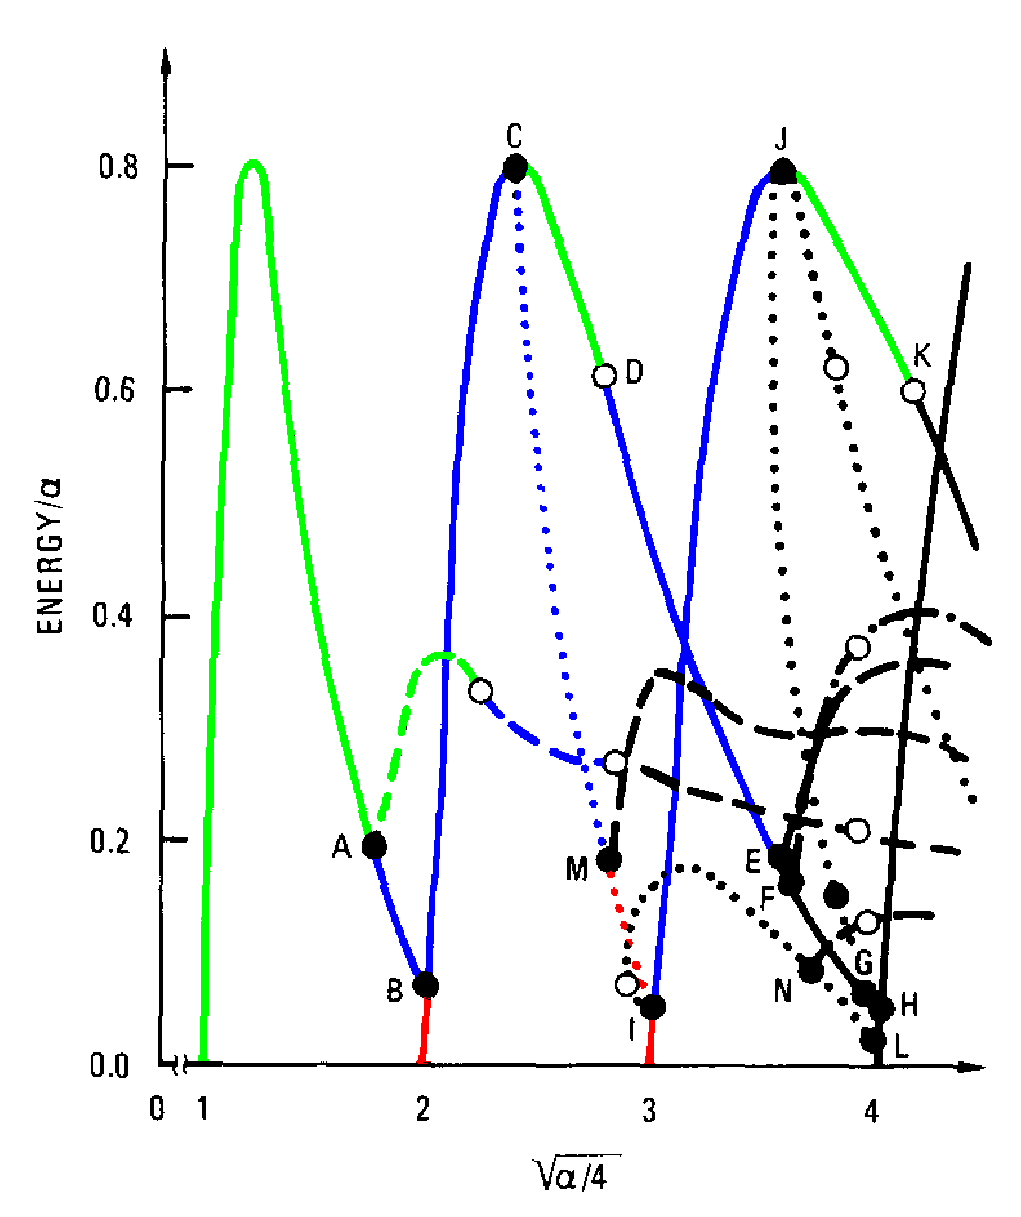
\includegraphics[width=0.5\textwidth, clip=true]
                {../rpo_ks/figsUnused/GreeneKimBifColor}
    % \vspace*{-5pt}
\caption[The ``energy'' of \eqva\ as a function of the bifurcation parameter]
        {
The ``energy'' of \eqva\ as a function of the bifurcation
parameter $\tildeL=\sqrt{\alpha}/2$, from \refref{ksgreene88}.
The solid curves denote $N$-cell solutions,
dotted curves GLMRT, the dash-dotted curve the
giant states, and dashed curves the propagating solutions.
Open circles indicate Hopf bifurcations.
We have color-coded the branches to reflect the number of unstable
eigenvalues (or complex pairs). Red: 2 unstable eigenvalues, Blue: 1
unstable eigenvalue, Green: stable. Solutions not
resolved in \refref{ksgreene88} or of no interest
to our present purposes have been left black.
        }
\end{figure}
%%%%%%%%%%%%%%%%%%%%%%%%%%%%%%%%%%%%%%%%%%%%%%%%%%%%%%%%%%%%%%%%%%

Greene and Kim study extends the earlier work\rf{Mks86,laquey74}
on the \KS\ \eqva\ and their bifurcations. The
bifurcation diagram \reffig{fig:GreeneKim} summarizes the results
relevant to the system sizes studied here.
    \PC{indicate Christiansen at al. and Lan and Cvitanovi\'c  choices of
    system size on the $\tildeL$ axis in \reffig{fig:GreeneKim}. Might
    require thinking - they are in the antisymmetric subspace, I tend to
    1/2 them but here one should not.}

For small $\alpha$ the only \eqv\ of the system is the constant solution
$y(x,t)=0$, which is globally attracting for $\tildeL=\sqrt{\alpha}/2<1$.
At $\tildeL=N$, with $N$ integer, the $N$th harmonic becomes unstable and
the constant solution bifurcates to the so called $N$-cell states. These
states contain only the multiples of the $N$th harmonic, {\ie} only the
components $a_N,a_{2N},...$ in our notation. Moreover, the $N$-cell
states are found to be symmetric (in our case, since $u=y_x$ they will be
antisymmetric). Greene and Kim show that symmetric solutions are \eqva,
not \reqva. At point $A$ in \reffig{fig:GreeneKim} the $1$-cell state
loses stability and bifurcates to a stable, asymmetric \reqv, which later
on becomes unstable through a Hopf bifurcation.
\PC{harmonize our notation with the ``$N$-cell state" notation}

At $\tildeL=2$ the system has become large enough that a $2$-cell \eqv\
appears. At point $B$ in \reffig{fig:GreeneKim} the $1$-cell branch
merges to the $2$-cell branch. In general each $N$-cell branch merges to
the corresponding $2N$-cell branch.

At point $C$ in \reffig{fig:GreeneKim} the $2$-cell state bifurcates to a
type of \eqv\ solution found by La Quey, Mahajan, Rutherford and
Tang\rf{laquey74} and generalized by Greene and Kim who refer to them as
GLMRT \eqva. GLMRT solutions are symmetric ($u(x)$ is antisymmetric) and
can be roughly described as long-wave distorted $N$-cell states.

The last type of solution identified in \refref{ksgreene88} appears at point $F$
in \reffig{fig:GreeneKim} and is called a
``giant" state because its amplitude grows as the system size increases.

According to the bifurcation diagram \reffig{fig:GreeneKim}, at the point
that corresponds to system size $\tildeL=\alpha^{1/2}/2=3.501$ studied
here, the {\eqva} we expect are the $2$- and $3$-cell states ($\EQV{2}$
and $\EQV{3}$ respectively), the GLMRT state that bifurcates from a
$3$-cell state at point $I$ ($\EQV{1}$), the \reqva\ that belong to the
branches starting at points $A$ ($\REQV{\pm}{1}$), and $M$
($\REQV{\pm}{2}$).

%%%%%%%%%%%%%%%%%%%%%%%%%%%%%%%%%%%%%%%%%%%%%%%%%%%%%%%%%%%%%%%%%
%\begin{figure}
%\begin{center}
%    %RESTORE? 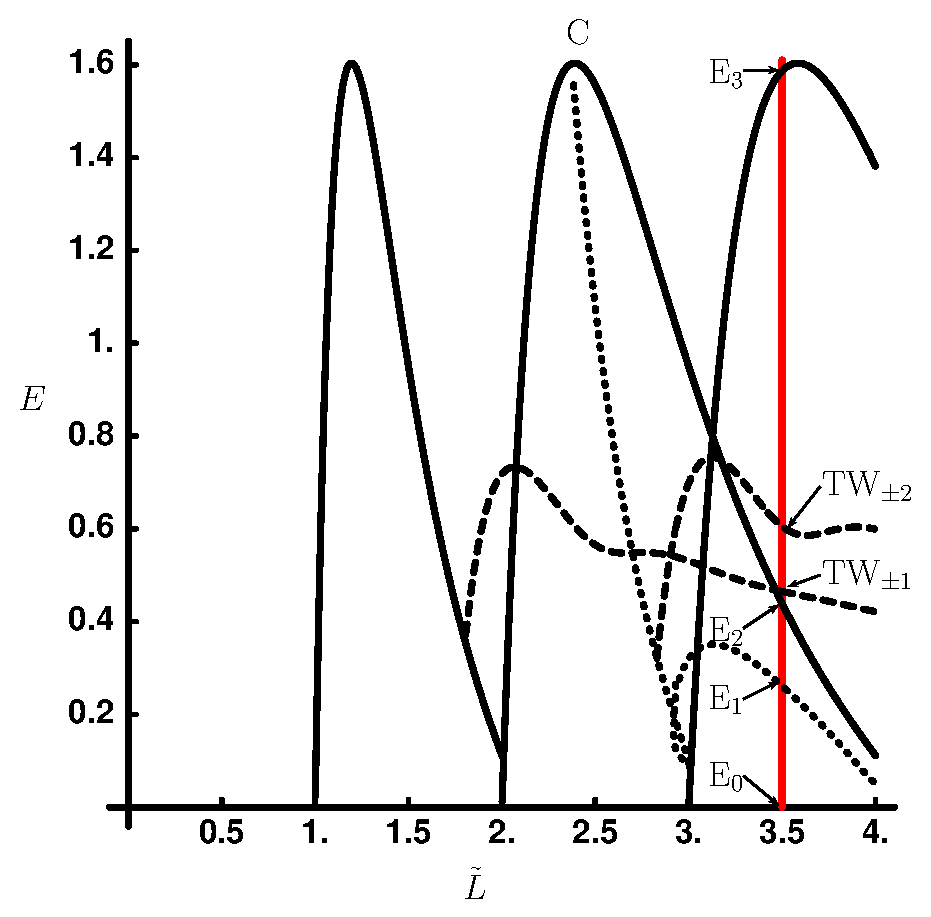
\includegraphics[width=0.5\textwidth]{ksBifDiag}
%\end{center}
%\caption[Bifurcation diagram for equilibria of Kuramoto-Sivashinsky eq.]
%    {
%    Bifurcation diagram for \eqva\ and \reqva\ of \KS\ system.
%    Shown is the 2c to GLMRT bifurcation and the GLMRT to $\REQV{\pm}{2}$ bifurcation,
%    points C and M in \rf{ksgreene88} respectively. The \reqv\ branch
%    is followed up to our system size.
%        }
%\end{figure}
%%%%%%%%%%%%%%%%%%%%%%%%%%%%%%%%%%%%%%%%%%%%%%%%%%%%%%%%%%%%%%%%%%%

\item[2011-09-15 Chao]
Stuck on understanding the $N$-cell states part Greene and Kim's paper.

In section 3.2, fourth line of the first paragraph, it is said ``The
nonlinear term $y_x^2$ couples only coefficients $C_{Ni}$.'' Why? This is
the key to the following calculation of eigenvalue matrix of N-cell
state.

\item[2011-09-17 Predrag] I believe this is explained in the beginning of
the same paragraph. It is a simple example of slicing; all \reqva\ trace
out circles in the full \statesp, one can use rotational \SOn{2} to
rotate the bifurcation problem into the $\sin Nx = 0$ plane, hence only $\cos$
terms matter. Not true in general, but true for bifurcations off the $y(x)=0$
\eqv; small perturbations are simply Fourier modes.


\item[2011-09-18] I can understand why we can assign $\sin Nx = 0$. What I actually
do not understand is why $y_x$ couples only coefficients with subscript $Ni$, multiples
of  $N$.

\item[2011-09-19 Evangelos] This is an important point. When I was a student
I was too lazy to follow in detail Greene and Kim's explicit calculation but
I remember finding a more elegant explanation in Kevrekidis, Nicolaenko
and Scovel\rf{KNSks90}. The real master of the general formalism is
Krupa\rf{Krupa90} but you will find hard to read his paper without sufficient
background in equivariant bifurcation theory (which I've found of no use so
far but is quite entertaining).

In my thesis, Sect. 5.1.7 in version 2, downloadable from chaosbook.org,
I've tried to explain how to understand the occurence and form of $N$-cell
states according to the equivariant branching lemma
(see \eg\ Hoyle\rf{hoyll06} or if you are brave Golubitsky and Stewart\rf{golubitsky2002sp}).
Everything was clear to me at the time of
writing and I was very satisfied I understood this. Now, some two years later I cannot
understand what I was talking about. I guess this is why no physicist
reads my thesis. If you are determined, there are enough pointers to the
original literature to guide you through the argument.

\item[2011-09-15 Chao]
In the following section 3.3, the third paragraph, it is said ``For each
subsector, $0<j<N/2$, every $N \times N$ block of the sine and cosine sectors of the
K matrix is reduced to a 2*2 block as follows:
\[
\left[
\begin{array}{cc}
K_{N(i-1)+j,N(i-1)+j}   &  K_{N(i-1)+j,Ni-j}\\
K_{Ni-j,N(i-1)+j}   &   K_{Ni-j,Ni-j}
\end{array}
\right]
\]
The diagonal elements contain $C_{k+l}$, or $C_{k-l}$ and have the same
sign in the cosine and the sine subsectors. Anti-diagonal elements
contain $C_{k+l}$ and change sign between the sine and cosine
subsectors.''

What I don't understand is that block of matrix $K$ is given in eq.~(9) in
the paper which is this. On the diagonal:
\[
V_{k,l}
=
l(k+l)
\left(
\begin{array}{cc}
-C_{k+l}   &  -S_{k+l}\\
-S_{k+l}   &   C_{k+l}
\end{array}
\right)
\]
Non-diagonal:
\[
V_{k,l}
=
l
\left[
\begin{array}{cc}
(k-l)C_{k-l}-(k+l)C_{k+l}   &  -(k-l)S_{k-l}-(k+l)S_{k+l}\\
(k-l)S_{k-l}-(k+l)S_{k+l}   &   (k-l)C_{k-l}+(k+l)C_{k+l}
\end{array}
\right]
\]
So diagonal blocks contain only $C_{k+l}$ while non-diagonal block may
contain both $C_{k+l}$ and $C_{k-l}$ which seems to contradict with the
statement quoted above.

Have been stuck on this for a while. Can anybody help me? Thanks.


\item[2011-09-17 Predrag] The main thing is to understand the bifurcation
diagram \reffig{fig:GreeneKim}, and then \emph{write it up it in the
notational conventions we use}, translating back and forth between their
article and ours can be a bit tedious. No need to reinvent the wheel, all
this has been done by Evangelos in
\emph{\HREF{http://www.chaosbook.org/projects/Siminos/thesis.pdf}
           {Thesis that Nobody Reads}}.
You will warm his heart if you convince him that you have read it, and it
has helped you. Go to siminos/thesis, latex thesis.tex, and read Sect.
5.1.7 there. Evangelos has redrawn bifurcation diagram
\reffig{fig:GreeneKim} in our convention, thesis figure 23. Or perhaps
read the same text (later version, perhaps edited compared to the thesis)
in Cvitanovi{\'c}, Davidchack and Siminos\rf{SCD07}, \refsect{s:SCD07},
or any of the many references there. So I do not think you need to
understand Greene notation, as long as you are able to reproduce the
important features of \reffig{fig:GreeneKim}.

Certainly reading Chapter 5 of  Lan thesis\rf{LanThesis}
should help (enter your notes into \refsect{s:LanThesis}).

\item[2011-09-18] OK. I'll explore their thesis:)

\item[2011-09-19 Evangelos] Certainly read Lan's thesis!

\end{description}

\subsection{Back in the saddle again:}
\label{s:KNSks90}

Notes on Kevrekidis, Nicolaenko and Scovel\rf{KNSks90}. A copy is in
\HREF{http://chaosbook.org/library/index.html}{ChaosBook.org/library}
(Predrag believes...).

\begin{description}

\item[2007-01-20 Evangelos]
Kevrekidis, Nicolaenko and Scovel\rf{KNSks90} study \KS\ system
steady state bifurcations and the role of symmetry in the
existence of structurally stable (relative) homoclinic and
heteroclinic cycles between unstable saddles. The form  of
the equation they use is essentially that of Greene and Kim but
with bifurcation parameter connected to our by
$\alpha=4\tilde{L}^2$.


They prove that the bifurcation of the trivial state $y=0$ to
an $N$-cell state is a pitchfork. They observe that when the
$1$-cell state losses stability at point $A$ the eigenvector
corresponding to the zero eigenvalue of the {\stabmat}
aligns itself with the direction of uniform translation of the
system which, due to the translational invariance of \KSe\,
also corresponds to a zero eigenvalue. Thus the algebraic
multiplicity of the zero eigenvalue is $2$ while its geometric
multiplicity is $1$. Using this fact and a local,
$O(2)$-equivariant, approximation to the center manifold they
prove that this type of bifurcation creates traveling waves.

In typical numerical simulations  a trajectory initiated along
the (single) unstable eigendirection of an \eqv\ $y$ of
the $2$-cell branch would eventually become attracted to the
$L/4$-translated \eqv\ $y'$. Those (relative) homoclinic
connections
\ES{In \refref{KNSks90} the characterization homoclinic
connection is used. Here we prefer (to invent?) the term
relative homoclinic to emphasize the fact that the \eqva\
are symmetry related.}
although structurally unstable in most dynamical systems, were
found to be persistent in \KS\ system with the afore-mentioned
behavior observed in the range from $\tilde{L}\simeq 2.009$ up
to $\tilde{L}\simeq 2.375$  where the $2$-cell state becomes
stable. The existence and robustness of the saddle connection
was explained as follows\ES{The following may not make perfect
sense without reading the paper, especially the notation. I've
start re-writing \KS\ symmetries section to incorporate
information about the invariant subspaces which hopefully will
explain it but my progress is very slow.}:  The unstable
manifold of $y$ lies on an invariant subspace $L$ of \KS\ flow,
which is the fixed set of the isotropy subgroup of $O(2)$
defined by reflection with respect to imaginary axis. The
action of the generator of $D(4)$ (which sends y to y') on $L$
is to send it to the invariant subspace $R_{1}$ which is the
fixed set of $Z(2)$ defined by complex conjugation. The
converse is also true, i.e. the action of $D(4)$ sends $R_{1}$
to $L$. Thus the unstable eigendirection of $y$, lying on $L$,
is sent on $R_{1}$ for the $L/4$-shifted point $y'$. The two
invariant subspaces $L$ and $R_{1}$ are orthogonal and thus the
point $y'$ has only stable eigendirections on $L$ and appears
as a sink on that subspace. This explains why the (relative)
homoclinic connections are structurally stable in \KS\ system.

In the range $\tilde{L}=2.00$ when the $2$-cell branch comes to
existence with two unstable eigendirections, up to $\tilde{L}
\simeq 2.009$ when it merges to the $1$-cell branch and losses
one of its unstable eigendirections, a heteroclinic loop exists
that connects $2$-cell to $1$-cell solutions. The analysis is
similar to the previous case.

 An important remark in \refref{KNSks90} is that the exact
 saddle connections were observed using a numerical integrator
 based on an explicit Galerkin spectral discretization of \KSe,
 irrespective of how close to the \eqv\ along the unstable
 manifold we start. On the contrary, when an FFT-based
 integrator was used, trajectories with initial condition along
 the unstable direction of $y$ would approach the homoclinic
 connection but fly away along the direction of the unstable
 manifold of $y'$ and follow an approximate (relative)
 homoclinic loop. This is attributed to the Galerkin truncation
 respecting the symmetries and possessing the same subspaces as
 the original equation restricted to the first $n$ modes
 \ES{We
 observe the second kind of behavior and we both use an FFT
 based integrator. I plan to quickly write a Galerkin integrator
 and check to see if we get an exact connection.}.
    %
\ES{Here I discuss Brown and Kevrekidis\rf{BrKevr96} MTW.}

\end{description}

\section{Chao's reading notes}
\label{s:KSreading}

\begin{description}
\item[2011-08-24 PC to Chao]
Read Siminos blog \refsect{sec:KSlit}, \emph{ \KS: literature survey}.
Other useful sources are Lan thesis, \refsect{s:LanThesis} and Siminos
thesis, \refsect{s:SiminosThesis}.
\end{description}


\subsection{Spatiotemporal chaos in terms of unstable recurrent patterns}
\label{s:Christiansen97}

In the initial work, the \statesp\ geometry and the natural measure for
this system have been
studied\rf{Christiansen97} in terms of unstable
periodic solutions restricted to the antisymmetric subspace of the
KS dynamics. Here are my notes on this Christiansen \etal\ paper.

\begin{description}

\item[2011-08-24 Chao]
The central work of using unstable recurrent patterns describing
spatiotemporal chaos is the search of \po s, especially unstable \po s.
Stable ones are not as important because they are attractive, within
their respective basins of attraction, and display no chaotic behavior.
The unstable ones are typically \emph{saddles}, with both unstable and
stable eigen-directions. In the unstable directions, they shoot out
neighboring points while in the stable directions they pull them in. Thus
dynamics is called ``hyperbolic'' because its linearized behavior is
hyperbolic. Taken together, the set of unstable \po s is the backbone of
chaotic behavior. While we cannot find \emph{all} unstable \po s of a
system (their number is infinite, growing exponentially with the period
of the orbit), we can decompose its dynamics as the combination of
influences of the near \po s.

This paper consists of 5 parts. I mainly focused on the 4th part:
one-dimensional visualization, which illustrate in detail how we find
\po\  and visulize them in low dimensions.

Here is my understanding of the whole process: First we choose a
\PoincSec\ in the full \statesp\ and let the dynamical system evolve for
a sufficiently long time to give us enough points on the section. This
enables us to define a return map $\PoincM$ for the section. Within the section,
iterating the map generates discrete-time \po s, which can be
found out exhaustively (in finite resolution) by utilizing symbolic
dynamics. Before we use symbolic dynamics, we have to build an intrinsic
arc-length coordinate system; for the parameter values studied here, close
to onset of chaos, this return map is approximately unimodal. This
situation is very special, due to only one direction of any \po\ being
unstable. The remaining ones (except for the single marginal eigenvalue
due to time invariance) are strongly contracting.
Since periodic points of a discrete time \po\ belong to the corresponding
continuous time \po\  in the full \statesp\, we can integrate from these
periodic points to recover the full space \po.

%%%%%%%%%%%%%%%%%%%%%%%%%%%%%%%%%%%%%%%%%%%%%%%%%%%%%%%%%%%%%%%%%%
\SFIG{return6a}
%%\includegraphics[width=0.65\textwidth]{../../../articles/vachtang/return6.ps}
{}{
The attractor of the \KS\ system,
% \refeq{expan}, %[2011-09-18 Predrag] \KSe\ have not been written down yet.
plotted as the $a_6$
component of the $a_1=0$ Poincar\'e section return map $\PoincM$. Here 10,000
Poincar\'e section returns of a typical trajectory are plotted. Also
indicated are the periodic points
${0}$, ${1}$, ${01}$ and ${10}$.
System size $ \tilde{L} = 2.89109$, $N=16$ Fourier modes truncation.
~~(From \refref{Christiansen97}.)
}{returnmap}
%%%%%%%%%%%%%%%%%%%%%%%%%%%%%%%%%%%%%%%%%%%%%%%%%%%%%%%%%%%%%%%%%%

Questions:

The third paragraph of part 4:
``The $i$th cycle point  $\arc_i$ is mapped onto its image $\arc_{\sigma i} =
f(\arc_i)$ where $\sigma i$ denotes  the label of the next periodic point in
the cycle.''


So that means $\sigma i$ is not meant to be $\arc_{i+1}$, right? Because the
order of different cycle points is given in following way: ``there exists
a fixed point which is not connected to the attractor (the point
$\overline{0}$ in \reffig{returnmap}) - we choose this fixed point as the
starting point and assign it number $1$. Point number $2$ is the periodic
point in the sample which is closest (in the full space) to this fixed
point, and the $n$th point is determined as the point which has the
minimum distance from the point number $n-1$ among all the periodic
points which have not yet been enumerated. Proceeding this way, we order
all the periodic points that we have found so far.''

So from this we could know that the order of periodic points on the
section is not the order of time evolution of these points. Right? But if
it is true, that seems to contradict with the illustration under figure
4?

\item[2011-08-30, 2011-09-18 Predrag]                            \toCB
For a general orbit we  label points in Poincar\'e section iteration by
\beq
\ssp_{n+1} = \PoincM(\ssp_n)
\ee{discrTime}
where $n=\{1,2,\cdots\}$ denotes the discrete time, and $\ssp$ is a point
in the \statesp\ $\pS \subseteq \reals^d$. For a periodic orbit of period
$n$ we use $\ssp_a$ where $a = \Ssym{1}\Ssym{2}\cdots\Ssym{n}$ is the
symbolic dynamics label of the cycle point  $\ssp_a$, and the dynamics
acts on the label as a cyclic permutation, $\sigma \ssp_a =
\Ssym{2}\cdots\Ssym{n}\Ssym{1}$
\beq
\ssp_{\Ssym{2}\cdots\Ssym{n}\Ssym{1}} =
    f(\ssp_{\Ssym{1}\Ssym{2}\cdots\Ssym{n}})
\,,
\ee{curvPO}
where the block $a=\Ssym{1}\Ssym{2}\cdots\Ssym{n}$ denotes the itinerary
of the periodic point $\ssp_a$ in the prime cycle $\pS_p$. For example,
11100-cycle point $\ssp_{11100}$ is mapped into next cycle point
$\ssp_{11001}$ which can be far away; spatial ordering of cycle points is
given by, for example, alternating binary trees.

In application at hand we discretize the 1-dimensional base segment of
the unstable manifold parametrized by arc-length $\arc$, so there is yet
another integer suffix which refers to a spatially ordered set of points,
for example
\beq
\arc_{j-1} < \arc_{j} < \arc_{j+1}
\,.
\ee{curvPO1}
In practice, we have two ways of populating the base segment by points -
either by running a long ergodic orbit and approximating each point on
the strange attractor by the nearest base segment point $\ssp(\arc)$,
labeled by the arc-length $\arc$, as is done in \refref{lanCvit07}, or by
threading a jagged line through the nearest periodic points, and adding
Euclidean distances between them to obtain $\arc$, as was originally done in
\refref{Christiansen97}. We prefer the former, as the latter approach of
necessity runs into ambiguities due to the fractal structure of a strange
attractor along the stable manifold directions, and one misses parts of
the base segment that are not reached by long-time ergodic dynamics.

The dynamics of close returns to the unstable manifold, approximated by
the nearest point on the manifold leads to return map
\beq
\arc_{n+1} = {f}(\arc_n)
\,,
\ee{curvTime}
where suffix $n=\{1,2,\cdots\}$ again denotes the discrete time, as in
\refeq{discrTime}.

\item[2011-9-19 CS]
The recurrent map has fractual structure in full state space and consequently in Poincare section. It means there are infinite many trajectories passing a finite area. For Kuramoto-Sivashinsky equation, the asymptotic dynamics is bounded in a low dimensionl space embedded in the full state space. In the special case here, the dynamics can be roughly considered as one dimensional because there is only one unstable direction and in other directions all the points are rapidly contracting. However, when we want to find periodic orbit, we have to consider the fractual structure becasue there are infinite many points here which may contain a lot of close periodic orbits(or relative periodic orbits).  Along the unstable eigendirection of a periodic orbit, we can do integral to construct a base segment. By parametrizing the segment by arc-length, we obtain a unimodel map. Then using symbolic dynamics we can found all the periodic cycles of this unimodel map, which provide very good initial guess of full state periodic orbits. The reason why the periodic cycles in the unimodel map is just a ``guess'' of periodic orbits in full state space is stated in the beginning that the recurrent map has very complicated fractual internal structure which is just ``roughly'' one dimensional, not exactly one dimensional. On the other hand, the unimodel map is exactly one dimensional and hence is just an approximation of the fractual thin dynamics. So we should start from this approximation to find the actual periodic points belonging to the real full-state-space periodic orbits.

The suffix n in equation 1.4 is discrete time, not in the order of arc-length. So the two equations do not contradict.

\noindent{\bf 2011-08-30 Predrag}
Can you try to add edited version of the above text to ChaosBook.org
smale.tex, section {\em Parametrization of invariant manifolds} which
clarifies this for the next reader? Maybe a drawing with a 3-cycle would
be helpful. Not sure...

\noindent
[ ] {\bf 2011-08-30 Predrag} mark this box once you have entered the
edits and discussed them with me.

%%%%%%%%%%%%%%%%%%%%%%%%%%%%%%%%%%%%%%%%%%%%%%%%%%%%%%%%%%%%%%%%%%
\SFIG{unfolded}
{}{
The return map $\arc_{n+1} = f(\arc_n)$ constructed from the images of periodic
points. The diamonds were obtained by using $34$ periodic points, the
dots were obtained by using $240$ periodic points. We have indicated the
periodic points $\overline{0}$, $\overline{1}$ and $\overline{01}$. Note
that the transverse fractal structure of the map shows when the number of
points is increased.
System size $ \tilde{L} = 2.89109$, $N=16$ Fourier modes truncation.
~~(From \refref{Christiansen97})
}{unfolded}
%%%%%%%%%%%%%%%%%%%%%%%%%%%%%%%%%%%%%%%%%%%%%%%%%%%%%%%%%%%%%%%%%%


\item[2011-08-24 Chao]
A prerequisite question is that from paragraph 2 to paragraph 3, the
phrase ``periodic points'' should mean the points on the 1-dimensional
return map, right? (or points on the $N-1$ dimensional Poincar\'e
section?) If so, since the 1-dimensional return map is a projection from
higher dimension, it could be that two different periodic points have the
same projection? What to do about that?

\item[2011-09-18 Predrag]                            \toCB
The return map \refeq{curvTime} is \emph{not a projection}: every point
on the 1-dimensional curve is a fully specified point in the full
\statesp, $\arc = \ssp(\arc)$, labeled by the arc-length $\arc$. That is precisely
why the approximation of the full dynamics by the iterates of the return
map is so powerful; the return map gives very good guesses for the
location of the next point in a cycle, which can then be pushed to
machine precision by the Newton or variational numerical algorithm used
in the \emph{full \statesp}.

\item[2011-08-24 Chao]
In figure 1, it is said `` The lower arrow indicates the kink where the
invariant set $A$ starts to overlap with $\theta SA$''. I don't understand
how the overlap of A and $\theta SA$ is connected to the kink in the
Feigenbaum tree. I don't have the intuition of how is it like that
``$A$ overlaps with $\theta SA$''. Can you show me some simple examples to
illustrate it pictorially so that I can have an intuitive feeling?

\noindent
[ ] {\bf 2011-08-25 Predrag} We have discussed this. Can you mark this
box once you have written up you what you understood. If things you have
learned are not written up now, they probably never will be written down.

\end{description}


\subsection{1-$d$ spatiotemporal chaos - A cyclist's view}
\label{s:LanThesis}

\begin{description}

\item[2011-09-17 PC to Chao]
Notes, questions \etc\ while studying
\HREF{http://www.cns.gatech.edu/~y-lan/index.html}{Yueheng Lan}
thesis\rf{LanThesis},
\emph{\HREF{http://www.cns.gatech.edu/~y-lan/thesis/index.html}
           {A cyclist's view}}.

\end{description}

\subsection{Unstable recurrent patterns in {\KS} dynamics}
\label{s:lanCvit07}

%\item[2011-08-24 PC to Chao]
Notes, questions \etc\ while studying Lan and Cvitanovi{\'c}\rf{lanCvit07}.

\begin{description}

\item[2011-09-03 Chao]
Comparing with the previous paper, \refsect{s:Christiansen97}, this paper
investigates a slightly larger \KS\ system which allows for more than one unstable
eigen-direction. I haven't got much more new things than I did in the previous
one because the idea in this paper is the same with the previous one.

\item[2011-09-12 Predrag] You are a harsh judge of men. Lan worked on
this over 6 years, and there is nothing new? That'll teach him to work
harder next time...
                            \toCB

\begin{itemize}
    \item
This slightly larger \KS\ system allows for more than one important \eqv\
solution, and is the first example of partitioning of its $\infty$\dmn\
\statesp\ into several neighborhoods.
    \item
It discusses the \eqv\ of KS on infinite domain, something not even mentioned
in \refref{Christiansen97}.
    \item
It finds an insanely long \emph{stable} \po, embedded in and visually
indistinguishable of the turbulence around it.
    \item
(Chao, fill in other novelties here...)
\end{itemize}

\item[2011-09-12 Chao]
Sorry for the improper wording. I meant that I could understand more
details in the paper only if I start compute myself such that I can have
more insight of the method and difficulties in this problem. Just that I
have not got yet, doesn't mean that it dosen't have novelties:)

\item[2011-09-03 Chao]

In page 4, section A, it is said ``We pick any point on a typical orbit
of (4). It corresponds to a loop in 3-d state space of (8) and so can be
used to initialize the search for an u(x) profile periodic on [0,L]''.
So, a point in the Fourier space periodic orbit is mapped into a loop in
real space? Don't feel like this is correct.

For your convenience,

equation (4):
\beq
\displaystyle\dot{a}_{k}
= (k/\tilde{L})^{2}(1-(k/\tilde{L})^{2})a_{k}
- (k/\tilde{L})\sum\nolimits^{+\infty}_{m=-\infty}a_{m}a_{k-m}
\ee{KSdiscr}

equation (8)
\beq u_x = v, v_x = w, w_x = u^2 - v -E
\eeq
For the rest part of the paper, I think I can well understand them only
if I start computation myself. I don't even know where to start to ask if
I don't go through the process. So I'll record the question here later if
I have any question in my own computation.
Plus, for further study and better understanding of this paper, I should
read \refrefs{ksgreene88}, [33]-[35] in particular.

\item[2011-09-15 Predrag] Citing [33]-[35] numbers from another paper is not
very helpful, to find out what they are one has to find that paper first...
please always refer to papers by our siminos.bib bibliography (I did it now
for Greene and Kim)


\item[2011-09-15 Predrag] Ref.~[33] is Christiansen and A. Politi\rf{chr95gen}:
we are not ready to read that one -
very important, but difficult and not needed in this project. The same
goes for Ref.~[35], Cvitanovi\'{c} and Hansen\rf{hansen1d}.

\item[2011-04-20, 2011-09-15 Predrag] You can get Ref.~[34],
Gilmore and Letellier\rf{GL-Gil07b}
{\em The Symmetry of Chaos}, from the CNS library. It only does the
invariant polynomial reduction (Siminos and I believe that is useless in
higher dimensions), but it is pretty good on discrete symmetries.
I would not give it high priority right now.

\end{description}


\subsection{Recurrent spatio-temporal structures
       in presence of continuous symmetries}
\label{s:SiminosThesis}

\begin{description}

\item[2011-09-17 PC to Chao]
Notes, questions \etc\ while studying Siminos thesis\rf{SiminosThesis}:
\emph{\HREF{http://www.chaosbook.org/projects/Siminos/thesis.pdf}
           {Thesis that Nobody Reads}}.


\end{description}


\subsection{60,000 \rpo s and no place to go}
\label{s:SCD07}

\begin{description}

\item[2011-08-24 PC to Chao]
Notes, questions, \etc, concerning
Cvitanovi{\'c}, Davidchack and Siminos\rf{SCD07},
\emph{On the \statesp\ geometry of the {\KS} flow}

\item[2011-09-03 Chao ]
This paper discussed in detail how symmetry simplifies the search for
\eqva, \reqva, \po s and \rpo s.. I
mainly focused on the first half and appendices which describe the idea
and computation methods. The rest of the paper is just details and
results of computation which I can only master by starting computing
myself.

\item[2011-09-12 Predrag]  You are a harsh judge of men. This is a
significant part of Siminos thesis, and it is `just details?'

\item[2011-09-03 Chao]
{\bf Appendix A:} I checked eq. (A.6) and it is correct. But the notion
of writing equation in Fourier transform operator is not so explicit.
That's why at first I was stuck. Eq. (A.5) is the same as eq. (4.2) in
Chaosbook. Here I rewrite (A.5) and (A.6) as (repeated indices summed over):
\bea
\dot{b}_k &=& \frac{\partial v_k(a)}{\partial a_j}b_j
\continue
v_k(a) &=& \dot{a}_k = (q^2_k - q^4_k)a_k - \frac{iq_k}{2}\sum\nolimits_ma_ma_{k-m}
\continue
\frac{\partial v(a)_k}{\partial a_j} &=&
(q^2_k - q^4_k) - \frac{iq_k}{2}\sum\nolimits_m(\delta_{mj}a_{k-m}+a_m\delta_{j,k-m})
\continue
&=& (q^2_k - q^4_k) - {iq_k}a_{k-j}
\,.
\label{KSstabMat1}
\eea
Combining the last two equations, we obtain:
\beq
\dot{b}_k = (q^2_k - q^4_k)b_k - iq_k\sum\nolimits_ja_{k-j}b_j
\,.
\label{KSstabMat2}
\eeq
The last term is discrete convolution of vector $a$ and $b$ in Fourier space,
which corresponds to component-wise product of two vectors in original
space due to Fourier transform. That is why it has the form in
(A.6).

We have to compute vector $\dot{b}_k$ because we have to observe how a
small deviation from the periodic orbit described by ${a_k,\dot{a}_k}$
evolves and integrate segment by segment(e.g. numerical integral) to
obtain Floquet Multipliers and thus obtain Jacobian matrix and Lyapunov
exponents.

Appendix C gives the searching algorithm of relative periodic orbits. I
got the idea, waiting to embark on real computation to knock down more
blockade.

\item[2011-10-16 CS]
From Appedix B, Ruslan's code and re-reading part of Chapter:Local Stability,
I learnt the first example on how to compute the Jacobian practically in the
``standard way''.

Here is a summary of the method:
We start the integration of ${a_k}$ and ${b_k}$ together according to
(A.4) and (A.6) respectively. The key point here is to recognize that
while ${a_k}$ is a component of the vector in Fourier space, $b_k$ is a
vector in tangent space, not a component of a vector. That's why we have
to extend the integration to N(N-1) dimensions. In the routine, the first
column of the N by N-1 matrix is vector $a$; from the second to last
column are real part and imaginary part of vectors ${b_k}$. We assign the
initial values of ${b_k}$ to be the ``unit'' vector(unit on both real and
imaginary axis) on each axis of the initial tangent space(which of course
is also the space of vector a). Then as the integration goes on, $a$
changes, more importantly, ${b_k}$ also changes. When it is done, $a$ get
the final value in the initial space and ${b_k}$ get the final value in
the final tangent space (which is just a relative frame with parallel axis
to the initial coordinate but origin fixed at point $a$). ${b_k}$ could
be rotated, stretched, or compressed. So the length and direction of
${b_k}$ may both change and are not orthogonal anymore. Then since the
initial value of ${b_j(0)}$ are actually orthogonal basis, the matrix
composed of all ${b_i(t)}$ is just the Jacobian because the elements are
$\partial{b_i(t)}/\partial{b_j(0)}$ which is exactly the definition of
Jacobian.

\item[2011-10-16 PC] The above summary looks right.

\end{description}
